\chapter{계속 배우면서 잊지 않기: continual learning의 문제 설정}
\label{bg:chapter-continual-learning}

\concept{continual-learning}{지속학습}은 데이터 분포가 한 번에 주어지지 않고 시간에 따라 도착할 때,
새 능력을 획득하면서 과거 능력도 유지하려는 설정이다. Sleep-time compute가 매일 또는 매 session 뒤
모델을 갱신한다면 자연스럽게 continual learning 문제가 된다. 단, 실제 agent stream은 benchmark처럼
``Task 1 종료, Task 2 시작'' 표지를 주지 않으며 사용자·사실·도구·정책 변화가 겹친다.

\section{왜 새 학습이 과거 능력을 지우는가}

한 파라미터 $\theta_j$가 과거 task A와 새 task B에 동시에 쓰인다고 하자. B의 loss를 줄이는 gradient가
A의 loss를 늘리는 방향이면 같은 update가 양쪽에 반대 효과를 낸다. 새 data만 반복하면 optimizer는
과거 data를 보지 못하므로 그 손실 증가를 감지하지 못한다. 이를 \concept{catastrophic-forgetting}{파국적
망각}이라 부른다. ``parameter capacity가 꽉 찼다''는 말과 같지는 않다. 충분한 파라미터가 있어도
optimization path와 sampling 때문에 잊을 수 있고, 반대로 작은 모델도 잘 선택한 replay와 isolation으로
오래 유지할 수 있다.

\concept{stability-plasticity}{안정성–가소성 dilemma}는 두 오류를 함께 본다.

\begin{itemize}
  \item 안정성만 높이면 이전 기능은 보존하지만 새로운 correction과 변화에 적응하지 못한다.
  \item 가소성만 높이면 최신 session에는 잘 맞지만 오래된 skill과 safety behavior가 무너진다.
\end{itemize}

Complementary Learning Systems 관점은 빠른 episodic store와 느린 cortical integration을 분리하고,
interleaved replay로 새 경험을 기존 구조에 통합한다 \parencite{mcclelland1995cls}. 이는 biological
sleep을 그대로 구현하라는 처방이 아니라, fast store가 제공하는 sparse episode와 slow learner가
요구하는 mixed training distribution이 다르다는 설계 basis다.

\section{성능 행렬로 retention과 transfer를 분리한다}

$R_{i,j}$를 task $j$까지 학습한 뒤 task $i$에서 측정한 성능이라 하자. 마지막 시점 평균 성능은

\begin{equation}
A_T=\frac{1}{T}\sum_{i=1}^{T}R_{i,T}
\end{equation}

이고, task $i$가 과거에 기록한 최고 성능에서 마지막 성능이 떨어진 양은

\begin{equation}
F_T=\frac{1}{T-1}\sum_{i=1}^{T-1}
\left(\max_{j\in\{i,\ldots,T-1\}}R_{i,j}-R_{i,T}\right)
\end{equation}

로 측정할 수 있다. \concept{backward-transfer}{후방 전이}는 새 학습이 과거 task를 개선하면 양수,
악화하면 음수인 방향성 지표다 \parencite{lopezpaz2017gem}. 평균 정확도 하나는 latest adaptation과
retention을 섞으므로 sleep controller 비교에 부족하다.

LLM memory에는 task label 대신 evaluation slice를 둔다. 예를 들어 user preference, stable personal
fact, time-varying fact, tool procedure, safety refusal, general capability, privacy non-leakage를 별도
행으로 만든다. 각 sleep version 뒤 이 행렬을 다시 측정해야 어느 축에서 얻고 잃었는지 보인다.

\begin{figure}[htbp]
  \centering
  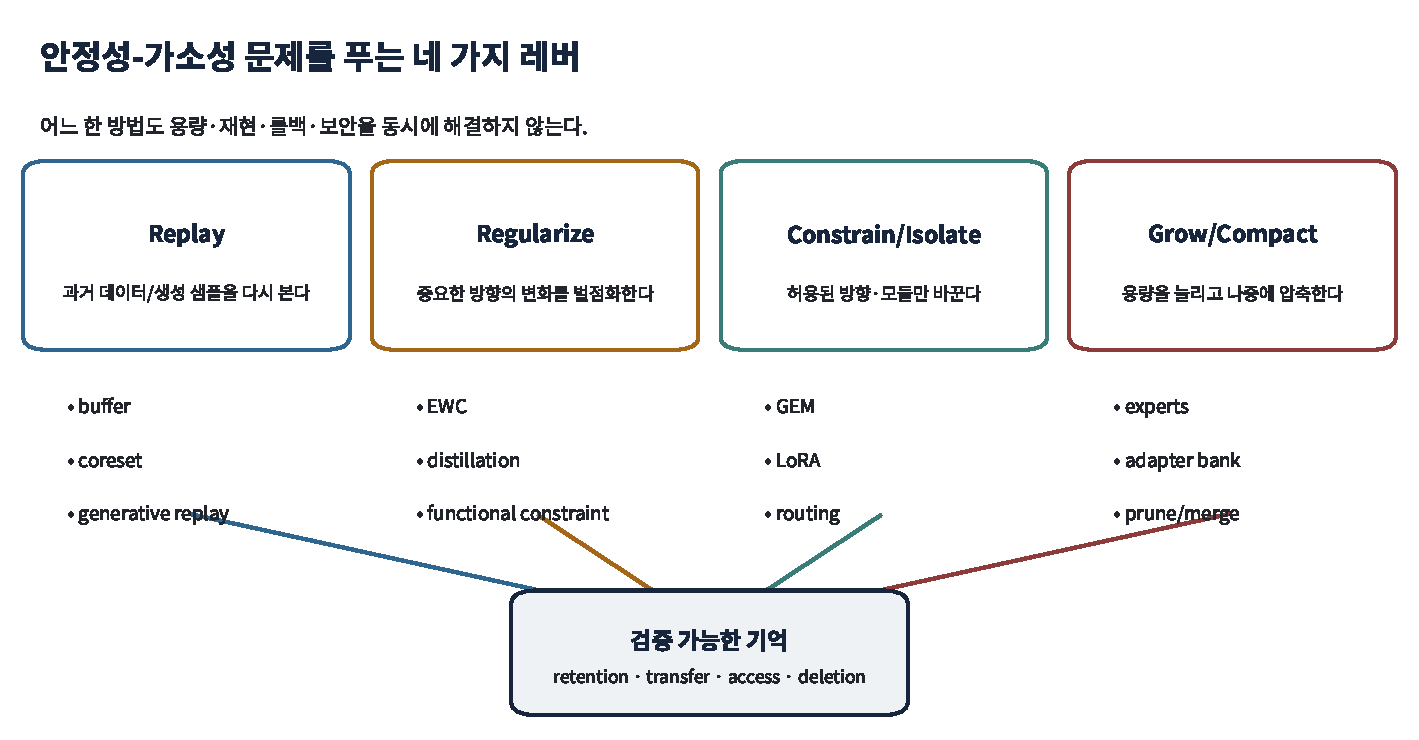
\includegraphics[width=0.95\textwidth]{figures/continual-learning-map.pdf}
  \caption{Continual-learning 방법을 replay, regularization, constraint/isolation,
  growth/compaction으로 나눈 지도. 네 계열 모두 별도 retention 평가와 publication gate가 필요하다.}
  \figsource{Original synthesis; SRC-STC-0002, SRC-STC-0003, SRC-STC-0004, SRC-STC-0007}{왼쪽의 네 방법 계열이 중앙의 후보 상태로 모이고, 평가와 출판을 통과해야 장기 기억으로 승격되는 흐름도.}
  \label{fig:bg-continual-map}
\end{figure}

\section{네 가족의 방법과 숨은 비용}

\begin{enumerate}
  \item \textbf{Replay}: 과거 data 또는 output을 다시 보여 준다. 가장 직접적이지만 storage, sampling,
        privacy와 data movement 비용을 낸다.
  \item \textbf{Regularization}: 과거에 중요한 parameter가 움직일 때 loss penalty를 준다. raw replay를
        줄일 수 있지만 중요도 state와 task boundary 가정을 요구한다.
  \item \textbf{Constraint/isolation}: 과거 loss를 나쁘게 하는 gradient를 투영하거나 parameter subspace를
        분리한다. interference는 줄지만 routing과 fragmentation이 생긴다.
  \item \textbf{Growth/compaction}: 새 module을 추가한 뒤 prune, merge, distill한다. plasticity는 높지만
        capacity가 단조 증가하지 않도록 별도 budget controller가 필요하다.
\end{enumerate}

\begin{table}[htbp]
\centering
\caption{Sleep 관점의 continual-learning 비교 질문}
\label{tab:bg-cl-comparison}
\small
\begin{tabularx}{\textwidth}{p{0.16\textwidth} X X X}
\toprule
계열 & 추가로 저장하는 것 & 주요 compute/I/O & 실패 질문 \\
\midrule
replay & raw/summary/example, metadata & storage read, forward/backward & 누가 buffer에서 밀려났는가? \\
regularization & old weights, importance & penalty compute, state read & 중요도 추정이 새 domain에도 맞는가? \\
projection & episodic gradient/reference & gradient dot product/solve & 제약이 plasticity를 봉쇄하는가? \\
isolation/growth & mask, adapter, expert, router & routing, fragmented reads & module 수와 cold state가 폭증하는가? \\
distill/compact & teacher snapshot, student & teacher inference + training & tail·provenance가 사라졌는가? \\
\bottomrule
\end{tabularx}
\end{table}

\section{온라인 평가와 shadow publication}

Sleep update 직후 사용자에게 바로 노출하면 과거 failure를 되돌릴 관찰 기간이 없다. 후보 version은
offline replay, held-out temporal test, adversarial scope test를 통과한 뒤 shadow traffic에서 current
version과 비교한다. 사용자별 adapter라 해도 global safety behavior와 다른 tenant non-leakage를 함께
검증한다. rollback unit은 optimizer step이 아니라 dataset manifest와 candidate artifact 전체다.

\begin{cautionbox}[Benchmarks의 task boundary를 그대로 믿지 말 것]
실서비스에서는 분포 변화, 사용자 correction, 일시적 event, 공격 input이 섞인다. task ID를 알고 있는
EWC/GEM 성능만으로 sleep system을 선택하면 trigger detection과 data contamination이라는 실제 비용을
누락한다. 연구 보고에는 boundary oracle 사용 여부와 buffer budget을 반드시 적는다.
\end{cautionbox}

Continual learning은 ``무한히 기억한다''는 약속이 아니다. 무엇을 잊어도 되는지, 어느 fidelity로
압축할지, 어떤 능력은 immutable base에 남길지 명시하는 bounded optimization이다. 다음 장은 그
mechanism과 capacity 한도를 수식으로 연결한다.
